\documentclass[10pt,a4paper]{article}
\usepackage[margin=0.8in]{geometry}
\usepackage[T1]{fontenc}
\usepackage{lmodern,microtype,booktabs,tabularx,graphicx,xcolor}
\usepackage{hyperref}
\hypersetup{hidelinks}
\setlength{\parindent}{0pt}\setlength{\parskip}{6pt}
\title{IDM-Viz: Exploratory Dependence-Change Detector Evaluation}
\author{Ahmed Bilal (23I-2581) \and Umar Behram (23I-2604)}
\date{16 November 2026}
\begin{document}\maketitle
\begin{abstract}
We evaluated a feature-only maximum pairwise-correlation-change score against the existing eight-feature plus three-PCA-coordinate KS alarm. On 30 fresh paired synthetic seeds, the new score detected the programmed C6 dependence change in all 30 onset windows, compared with 16 of 30 for KS/PCA. It selected the programmed pair (X0,X1) in all 30 seeds. The gain came with higher stationary alarm burden: 1.70 versus 0.83 alarms per 24 batches. This exploratory result supports a targeted complement for the tested dependence intervention; it does not establish general dependence detection or harm prediction.
\end{abstract}
\section{Protocol and scope}
The statistic is the maximum absolute off-diagonal difference between current-batch and historical-reference Pearson correlation matrices. The reference is the final 1,000 rows of the canonical 2,000-row reference partition. A single 95th-percentile higher-rule threshold was chosen using 720 stationary development batch scores from seeds 930000--930029. The frozen threshold is 0.165740. Evaluation used seeds 930100--930129 and all seven original conditions, with 24 batches of 500 rows. The same streams were scored by a recomputed training-only standardized KS family over eight original features and three training-fitted PCA coordinates, with Holm correction at 0.05.

The study was designed after the previous 1,500-seed study revealed weak C6 sensitivity. It is therefore an exploratory follow-up, despite using fresh evaluation seeds. No labels enter either detector. The maximizing pair is descriptive and is not a causal explanation.
\section{Results}
\begin{table}[ht]\centering\small
\caption{Onset detection frequency by condition. Onset is batches 9--12; values are proportions over 30 seeds.}
\begin{tabular}{lrr}\toprule Condition & Correlation & KS/PCA \\\midrule
C0 & 0.400 & 0.133 \tabularnewline
C1 & 0.400 & 1.000 \tabularnewline
C2 & 0.400 & 1.000 \tabularnewline
C3 & 0.400 & 0.133 \tabularnewline
C4 & 0.400 & 0.133 \tabularnewline
C5 & 0.400 & 0.133 \tabularnewline
C6 & 1.000 & 0.533 \tabularnewline
\bottomrule\end{tabular}\end{table}

For C6, the paired detection-rate difference was 0.467 (95\% seed-bootstrap interval [0.300, 0.633]; 2,000 resamples). The correlation detector selected pair (X0,X1) during an alarm in 30/30 C6 onset windows. This is exact recovery of the programmed pair in this generator, not general feature-pair localization.

On stationary C0, the correlation score produced 1.70 alarms per 24 batches (70.8 per 1,000 batches) versus 0.83 (34.7 per 1,000) for KS/PCA. The paired difference was 0.87 alarms per stream (95\% seed-bootstrap interval [0.40, 1.37]). The correlation detector's pre-onset stream false-alarm rate in C0 was 40\% versus 16.7\% for KS/PCA. The threshold's per-batch development quantile did not control stream-level false alarms to the comparator's burden.

\begin{figure}[ht]\centering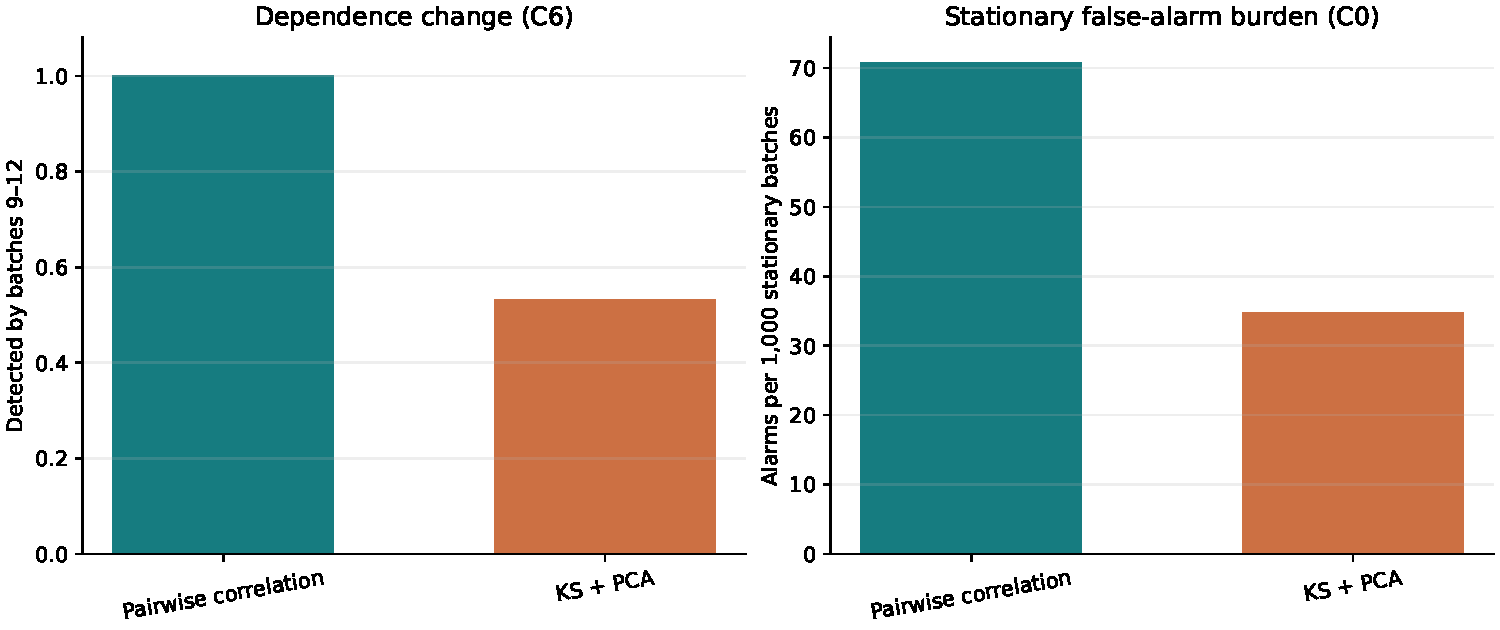
\includegraphics[width=.9\linewidth]{dependence_tradeoff.pdf}
\caption{Onset detection and stationary alarm burden. The detector improves sensitivity for C6 while increasing alarms under stationarity.}\end{figure}
\section{Interpretation and limits}
The result justifies retaining pairwise correlation evidence as a separate targeted signal in this synthetic setting, with explicit alert-burden costs. It does not show that correlation is the cause of model harm, that alarms predict loss, or that operators benefit. C1/C2 marginal shifts remain more readily detected by the KS/PCA family. The max-pair statistic can miss higher-order dependence changes and its threshold needs a burden-aware calibration rule before deployment. Only one synthetic dependence mechanism, one learner-independent input stream and 30 fresh seeds were evaluated.

\section{Reproduction}
From the repository root, run development before evaluation:
\begin{verbatim}
python scripts/run_phase3_dependence_extension.py --mode development `
  --out results/dev_NEW
python scripts/run_phase3_dependence_extension.py --mode final `
  --threshold-file results/dev_NEW/threshold.json `
  --out results/final_NEW
python scripts/evaluate_phase3_dependence_extension.py --run results/final_NEW
\end{verbatim}
The actual development and final CSVs, threshold locks, source hashes and validation receipt accompany this report.\end{document}
